\documentclass{article}
\usepackage{amsthm}
\usepackage{amsmath}
\usepackage{graphicx}
\usepackage{color}
\usepackage{subfig}
\usepackage{physics}
\graphicspath{ {figures/} }

\begin{document}

\begin{figure}

  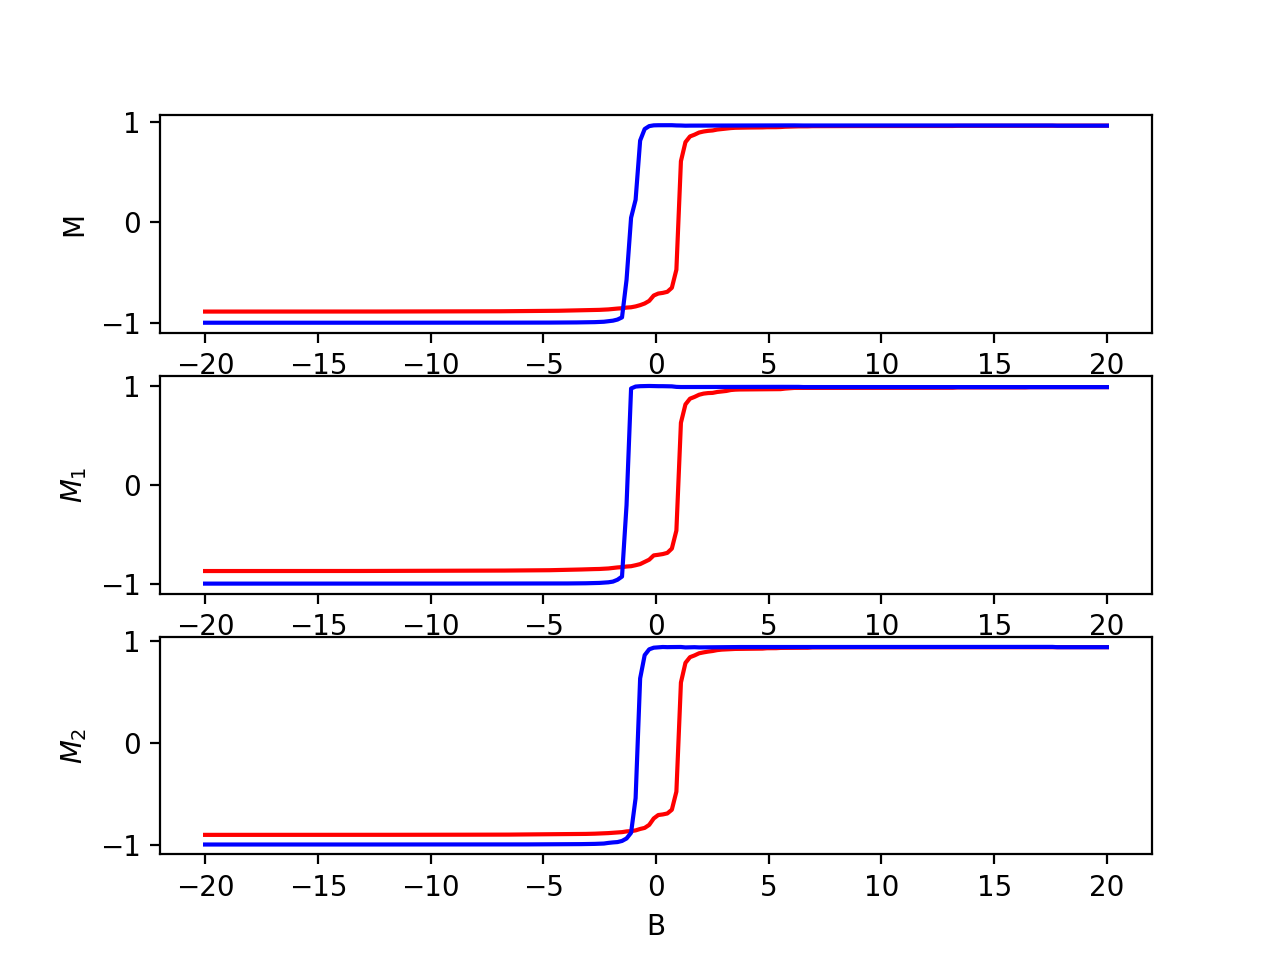
\includegraphics[width=\textwidth]{figures/magvb_b_20_k_0.png}

\caption{Magnetization vs external B field strength for $10 \times 10$ lattice at temperature $T = .001$. $B$ ranges from $-20$ to $20$ in $.2$ intervals. $k_{1} = k_{2} = 0$.
}
\end{figure}

\begin{figure}

  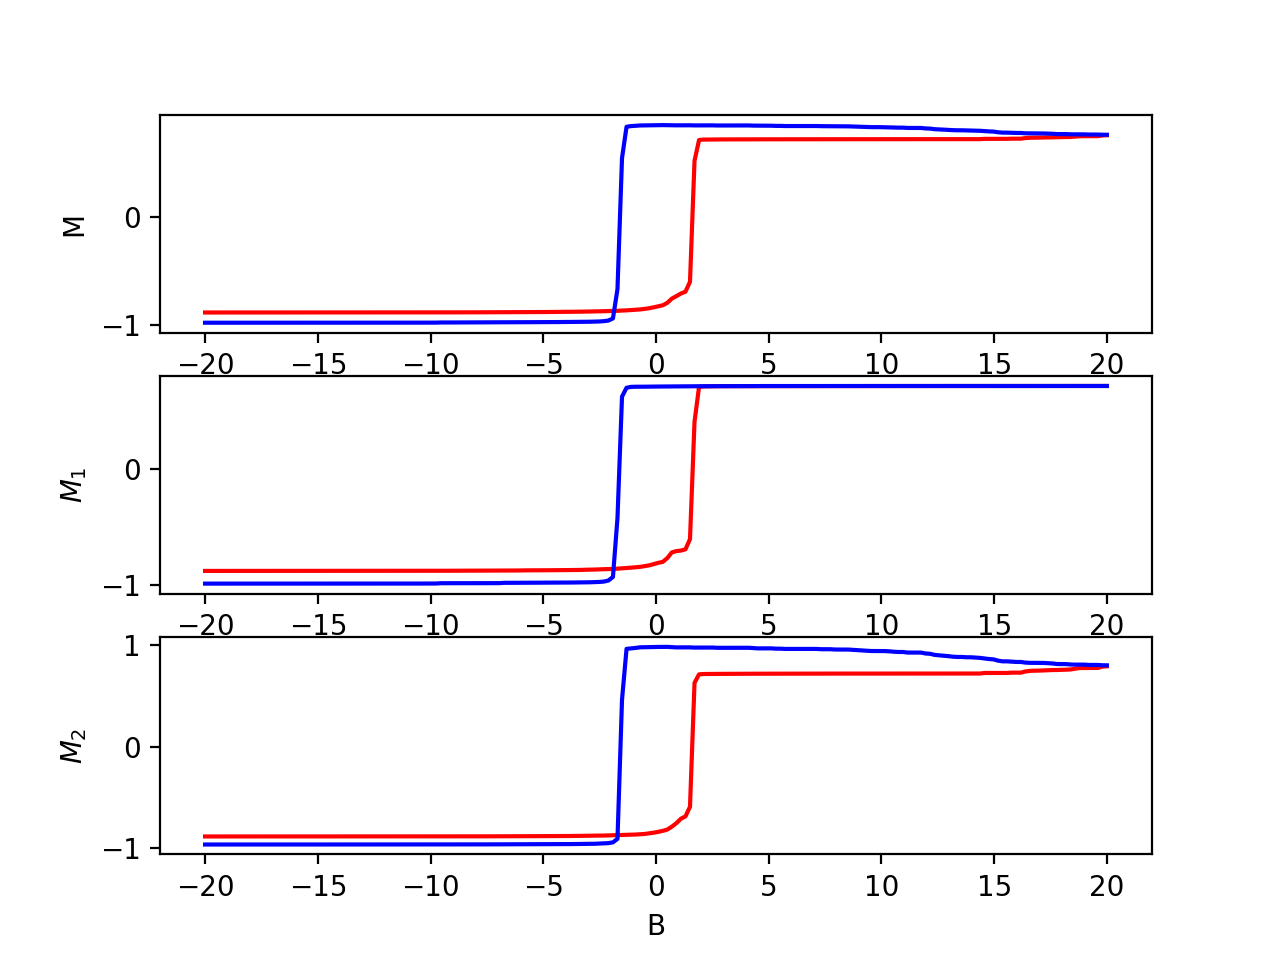
\includegraphics[width=\textwidth]{figures/magvb_b_20_k_p5.png}

\caption{Magnetization vs external B field strength for $10 \times 10$ lattice at temperature $T = .001$. $B$ ranges from $-20$ to $20$ in $.2$ intervals. $k_{1} = k_{2} = .5$.
}
\end{figure}

\begin{figure}

  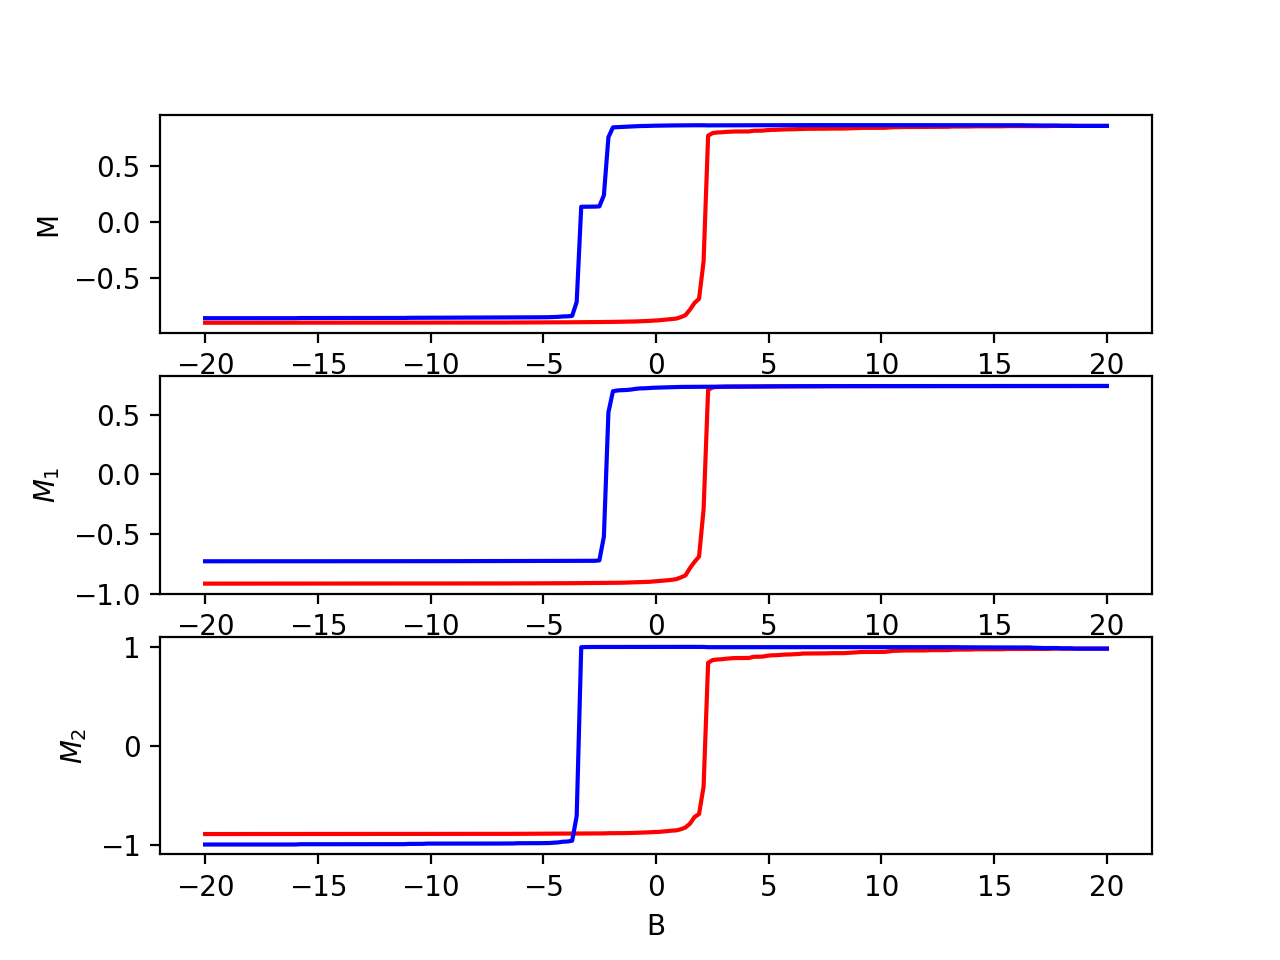
\includegraphics[width=\textwidth]{figures/magvb_b_20_k_1.png}

\caption{Magnetization vs external B field strength for $10 \times 10$ lattice at temperature $T = .001$. $B$ ranges from $-20$ to $20$ in $.2$ intervals. $k_{1} = k_{2} = 1$.
}
\end{figure}
\begin{figure}

  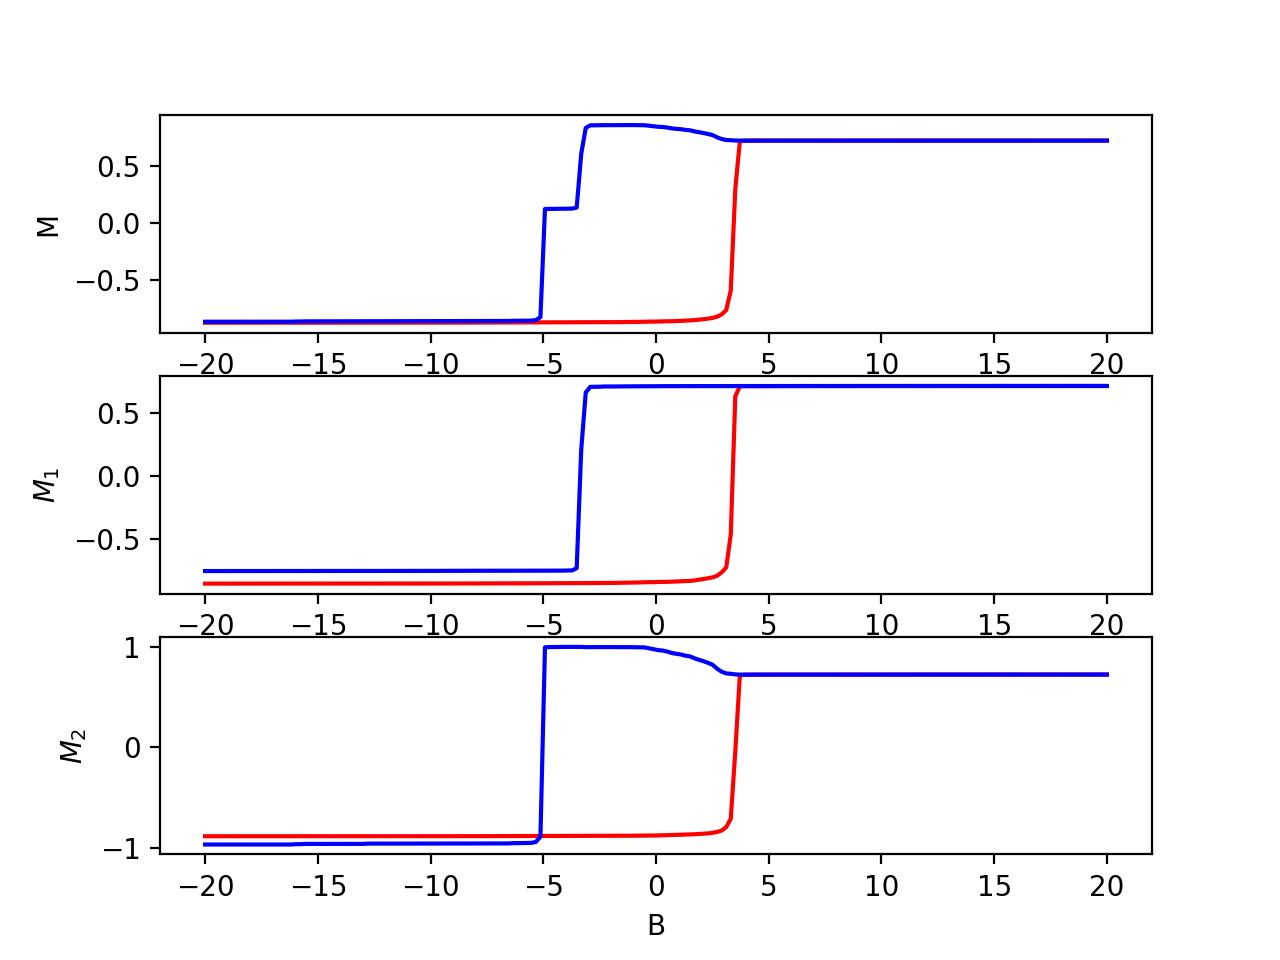
\includegraphics[width=\textwidth]{figures/magvb_b_20_k_2.png}

\caption{Magnetization vs external B field strength for $10 \times 10$ lattice at temperature $T = .001$. $B$ ranges from $-20$ to $20$ in $.2$ intervals. $k_{1} = k_{2} = 2$.
}
\end{figure}
\end{document}
